\documentclass[a4paper, 11pt]{article}
\usepackage{graphicx}
\usepackage{amsmath}
\usepackage[pdftex]{hyperref}
\usepackage{subcaption}

% Lengths and indenting
\setlength{\textwidth}{16.5cm}
\setlength{\marginparwidth}{1.5cm}
\setlength{\parindent}{0cm}
\setlength{\parskip}{0.15cm}
\setlength{\textheight}{22cm}
\setlength{\oddsidemargin}{0cm}
\setlength{\evensidemargin}{\oddsidemargin}
\setlength{\topmargin}{0cm}
\setlength{\headheight}{0cm}
\setlength{\headsep}{0cm}

\renewcommand{\familydefault}{\sfdefault}

\title{Machine Learning 2015: Project 1 - Regression Report}
\author{jo@student.ethz.ch\\ sakhadov@student.ethz.ch\\ kevinlu@student.ethz.ch\\}
\date{\today}

\begin{document}
\maketitle

\section*{Experimental Protocol}
We used split-training (train on 80\%, test on 20\%) and ten fold cross-validation to select the best models. \\
To better understand the data and feature importance, we used two different plotting methods. Firstly, we plotted every combination of two features and the class on the third axis. With this we could see that there are some outliers in the data, and we could set the thresholds for the outliers visually. From figure \ref{2Features} we can see that we can set the threshold to 4 on the frequency 1, because the points beyond this limit are clearly to far away from the centers.\\ 
Furthermore, we plotted all combinations of three features on a 3D graph. With this technique we could examine the importance of each feature. Figure \ref{3Features} shows that the frequency 5 has probably no impact on the labels, because the means of different classes lay roughly on the same height.


\begin{figure}[!b!]
 \centering 
\begin{subfigure}[b]{0.4\textwidth}
	\centering
	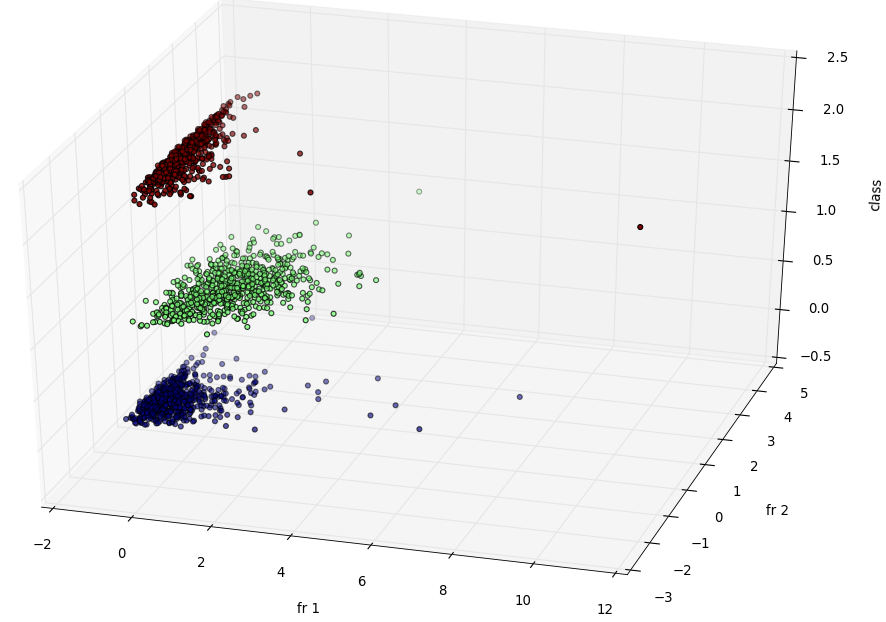
\includegraphics[width=\textwidth]{2_features.png} 
	\caption{}
	\label{2Features}
\end{subfigure}
\hfill
\begin{subfigure}[b]{0.4\textwidth}
	\centering
	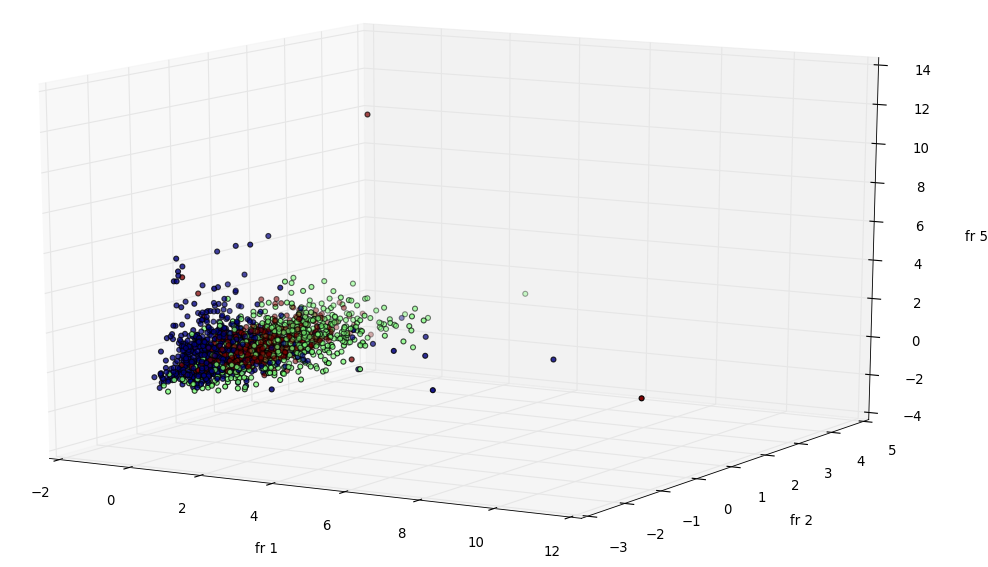
\includegraphics[width=\textwidth]{3_features.png} 
	\caption{}
	\label{3Features}
\end{subfigure}
\caption{We used different visualization strategies to better understand the data. On the left two different features are plotted on the horizontal axis and the labels on the vertical axis. On the right three different features are plotted on three axis and the data points have the color of its class.}
\end{figure}

\section{Tools}
We used Python 2 with the machine learning library \textit{scikit-learn} and \textit{numpy}. Also, for the \textit{artificial neural network} approach we used a Python library called \textit{Lasagne}.

\section{Algorithm}
\textit{Random forest regression} builds multiple decision trees during training (using randomization). Each tree makes a prediction and the average value is taken as the final result.

\section{Features}
We did not construct any new features, as it did not improve the performance in the settings we chose.

\section{Parameters}
Parameters were found using grid search. For every possible set of parameters 3-fold cross-validation was performed to find the best generalizing parameters. To validate the model afterwards, a 10-fold cross-validation was applied together with a split-test, where we trained on 80\% of the data and tested on the other 20\%.

\section{Lessons Learned} In an alternative approach, we tested an \textit{artificial neural network} (ANN). However, it did not perform better than the \textit{random forest regressor}. Neural networks may be better suited for a case where the number of features is large and the explicit knowledge about separate features is very limited, for instance face recognition.

\end{document}
